We first inspect the clusters based on the average values of meaningful
features (see \fgrref[A]{fig:clusterFeatVar}; \citealp{Kennedy2021}). We
(1) see that for some variables the features are generally stronger in
separating the clusters (e.g., `how cooperative an interaction was'
compared to `attitudes towards the Dutch'). Additionally, we see that
(2) within the variables some features are better at distinguishing
clusters (e.g., median of well-being vs.~MAC of well-being).We then
inspect the clusters with a focus on the features (see
\fgrref[B]{fig:clusterFeatVar}). While this is the same data as for the
variable focus, we can see more clearly that some features are better at
distinguishing the clusters across variables (e.g., mean and median
compared to auto correlations). This offers some information on which
features were are most important in understanding the two extracted
groups.

\begin{figure}[!ht] %hbtp
  \caption{Cluster Group Comparisons based on Features and Variables}
  \label{fig:clusterFeatVar}
  \centering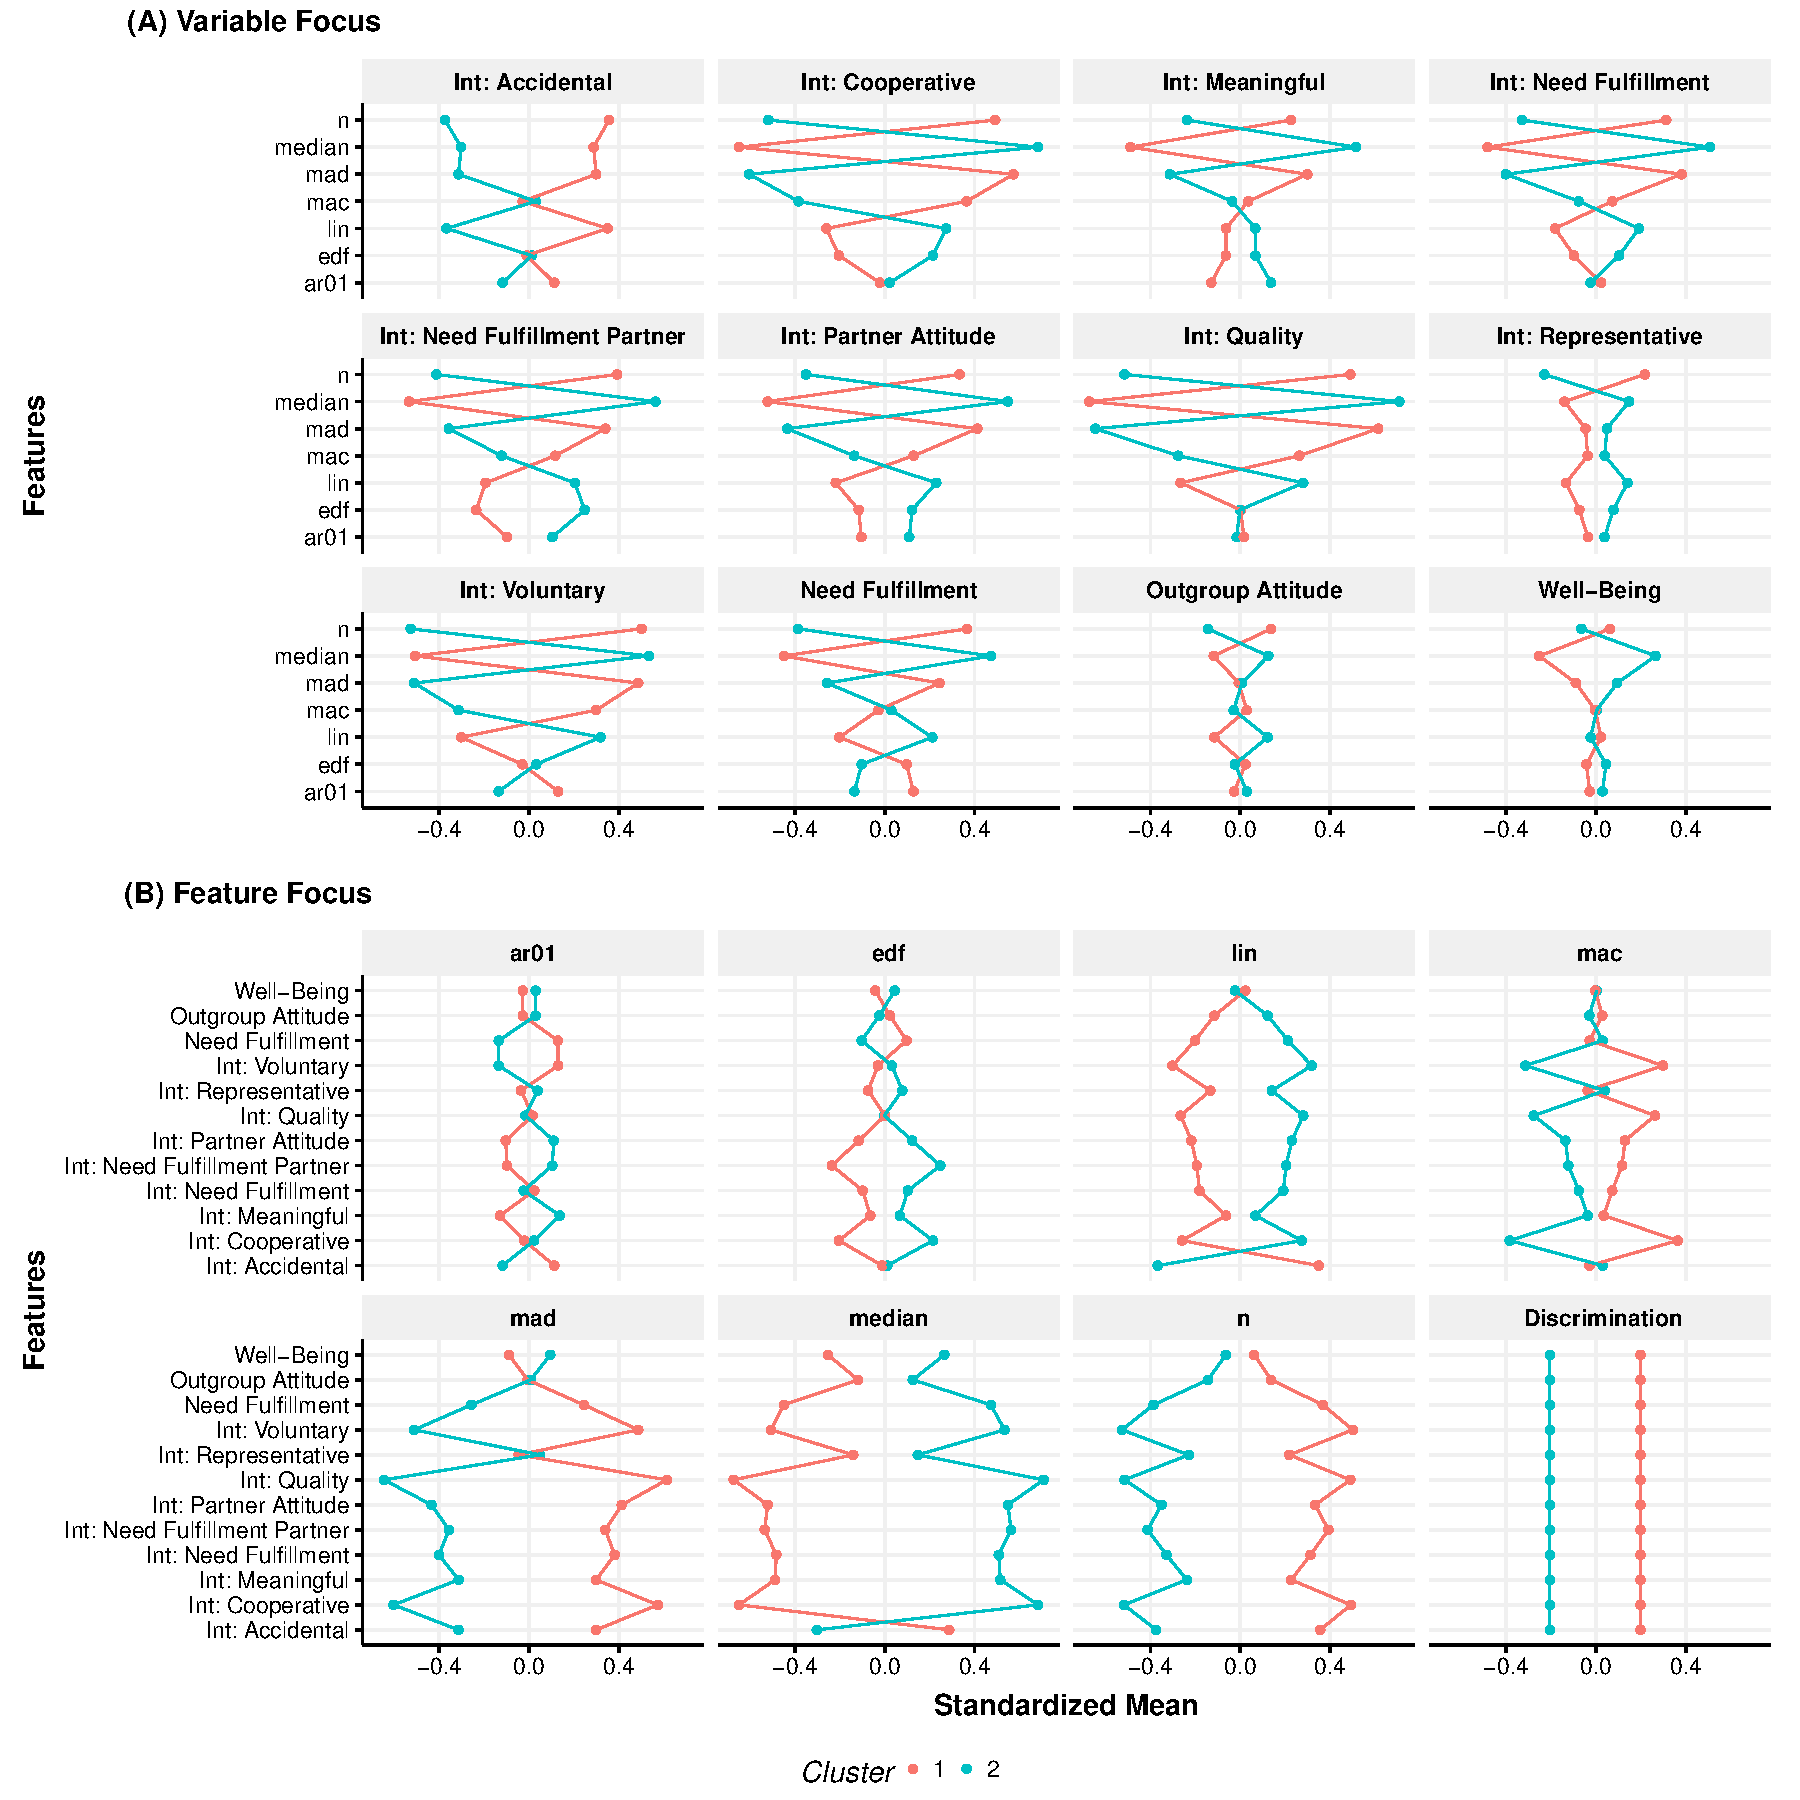
\includegraphics[width=\textwidth]{figures/clusterFeatVarComb.pdf}
  \caption*{Note: \\
  Within the "(B) Feature Focus" subplot, the 'n' and 'Discrimination' comparison variables were not part of the original time series clustering.}
\end{figure}

In the second step, we look at prototypical trajectories of the
clusters. For k-means clustering it is often recommended to use the
average over time of the responses within the cluster
\citep[see \fgrref{fig:clusterTs}][]{niennattrakul2007}\footnote{It is important to note, however, that direct comparability can be a concern, and often times some subset selection or nonlinear alignment is necessary \citep[e.g.,][]{gupta1996}. Additionally, finding cluster prototypes is often substantially easier with embedded clustering methods because in many cases a cluster-level model is estimated as part of the expectation–maximization procedure \citep[e.g.,][]{denteuling2021}. For medoid-based clustering algorithms, a common approach is simply using cluster medoid as the prototype \citep{kaufman1990}.}.
Immediately striking are the mean differences, where participants in the
second cluster had more meaningful and fulfilling outgroup interactions
also consistently reported more voluntary and cooperative interactions
but less accidental and involuntary interactions. The same cluster also
reported an increase in need fulfilling interaction over the 30 day
period and an increase in interactions that were representative of the
outgroup. Whereas the other cluster showed a decrease in voluntary,
cooperative, and positive interactions over the 30 days. This
`deterioration' cluster also saw a decrease in general need fulfillment
and experienced well-being over the 30 days (see
\fgrref[B]{fig:clusterTs}). We also see that while interaction
representativeness, outgroup attitudes, well-being are relatively stable
for both clusters, the deteriorating cluster also showed substantially
higher variablity and instability over time (also see
\fgrref[A]{fig:clusterTs}).

Finally, we can also assess the clusters across other person-level
variable \citep[e.g.,][]{monden2022}. This out-of-feature comparison
allows us to check for data artifacts, as well as check whether the
developmental clusters are associated with important social markers and
individual differences. To illustrate artifact checks, we added the
number of measurements into the comparison and find that the
participants in the detereoration cluster on average completed more ESM
surveys and reported on more intergroup interactions than the cluster
with the more positive interactions (see \fgrref[B]{fig:clusterTs}).
While this difference could indicate that the clusters might not
entirely be comparable in the response patterns, we can find some relief
in our data exclusion procedures during which we ensured that the
general time frame and completion rates were not too dissimilar. To
illustrate the utility of individual differences, we compare the two
samples in terms of the participants' self-reported discrimination
experiences in the Netherlands (measured during the post-measurement).
\fgrref[B]{fig:clusterTs} illustrates that participants in the
deteriorating cluster reported substantially higher levels of everyday
discrimination. Thus, both intensive longitudinal and cross-sectional
variables that were not included in the original clustering step can be
used to explore and understand the cluster differences in more detail.

\begin{figure}[!ht] %hbtp
  \caption{Cluster Group Comparisons over time}
  \label{fig:clusterTs}
  \centering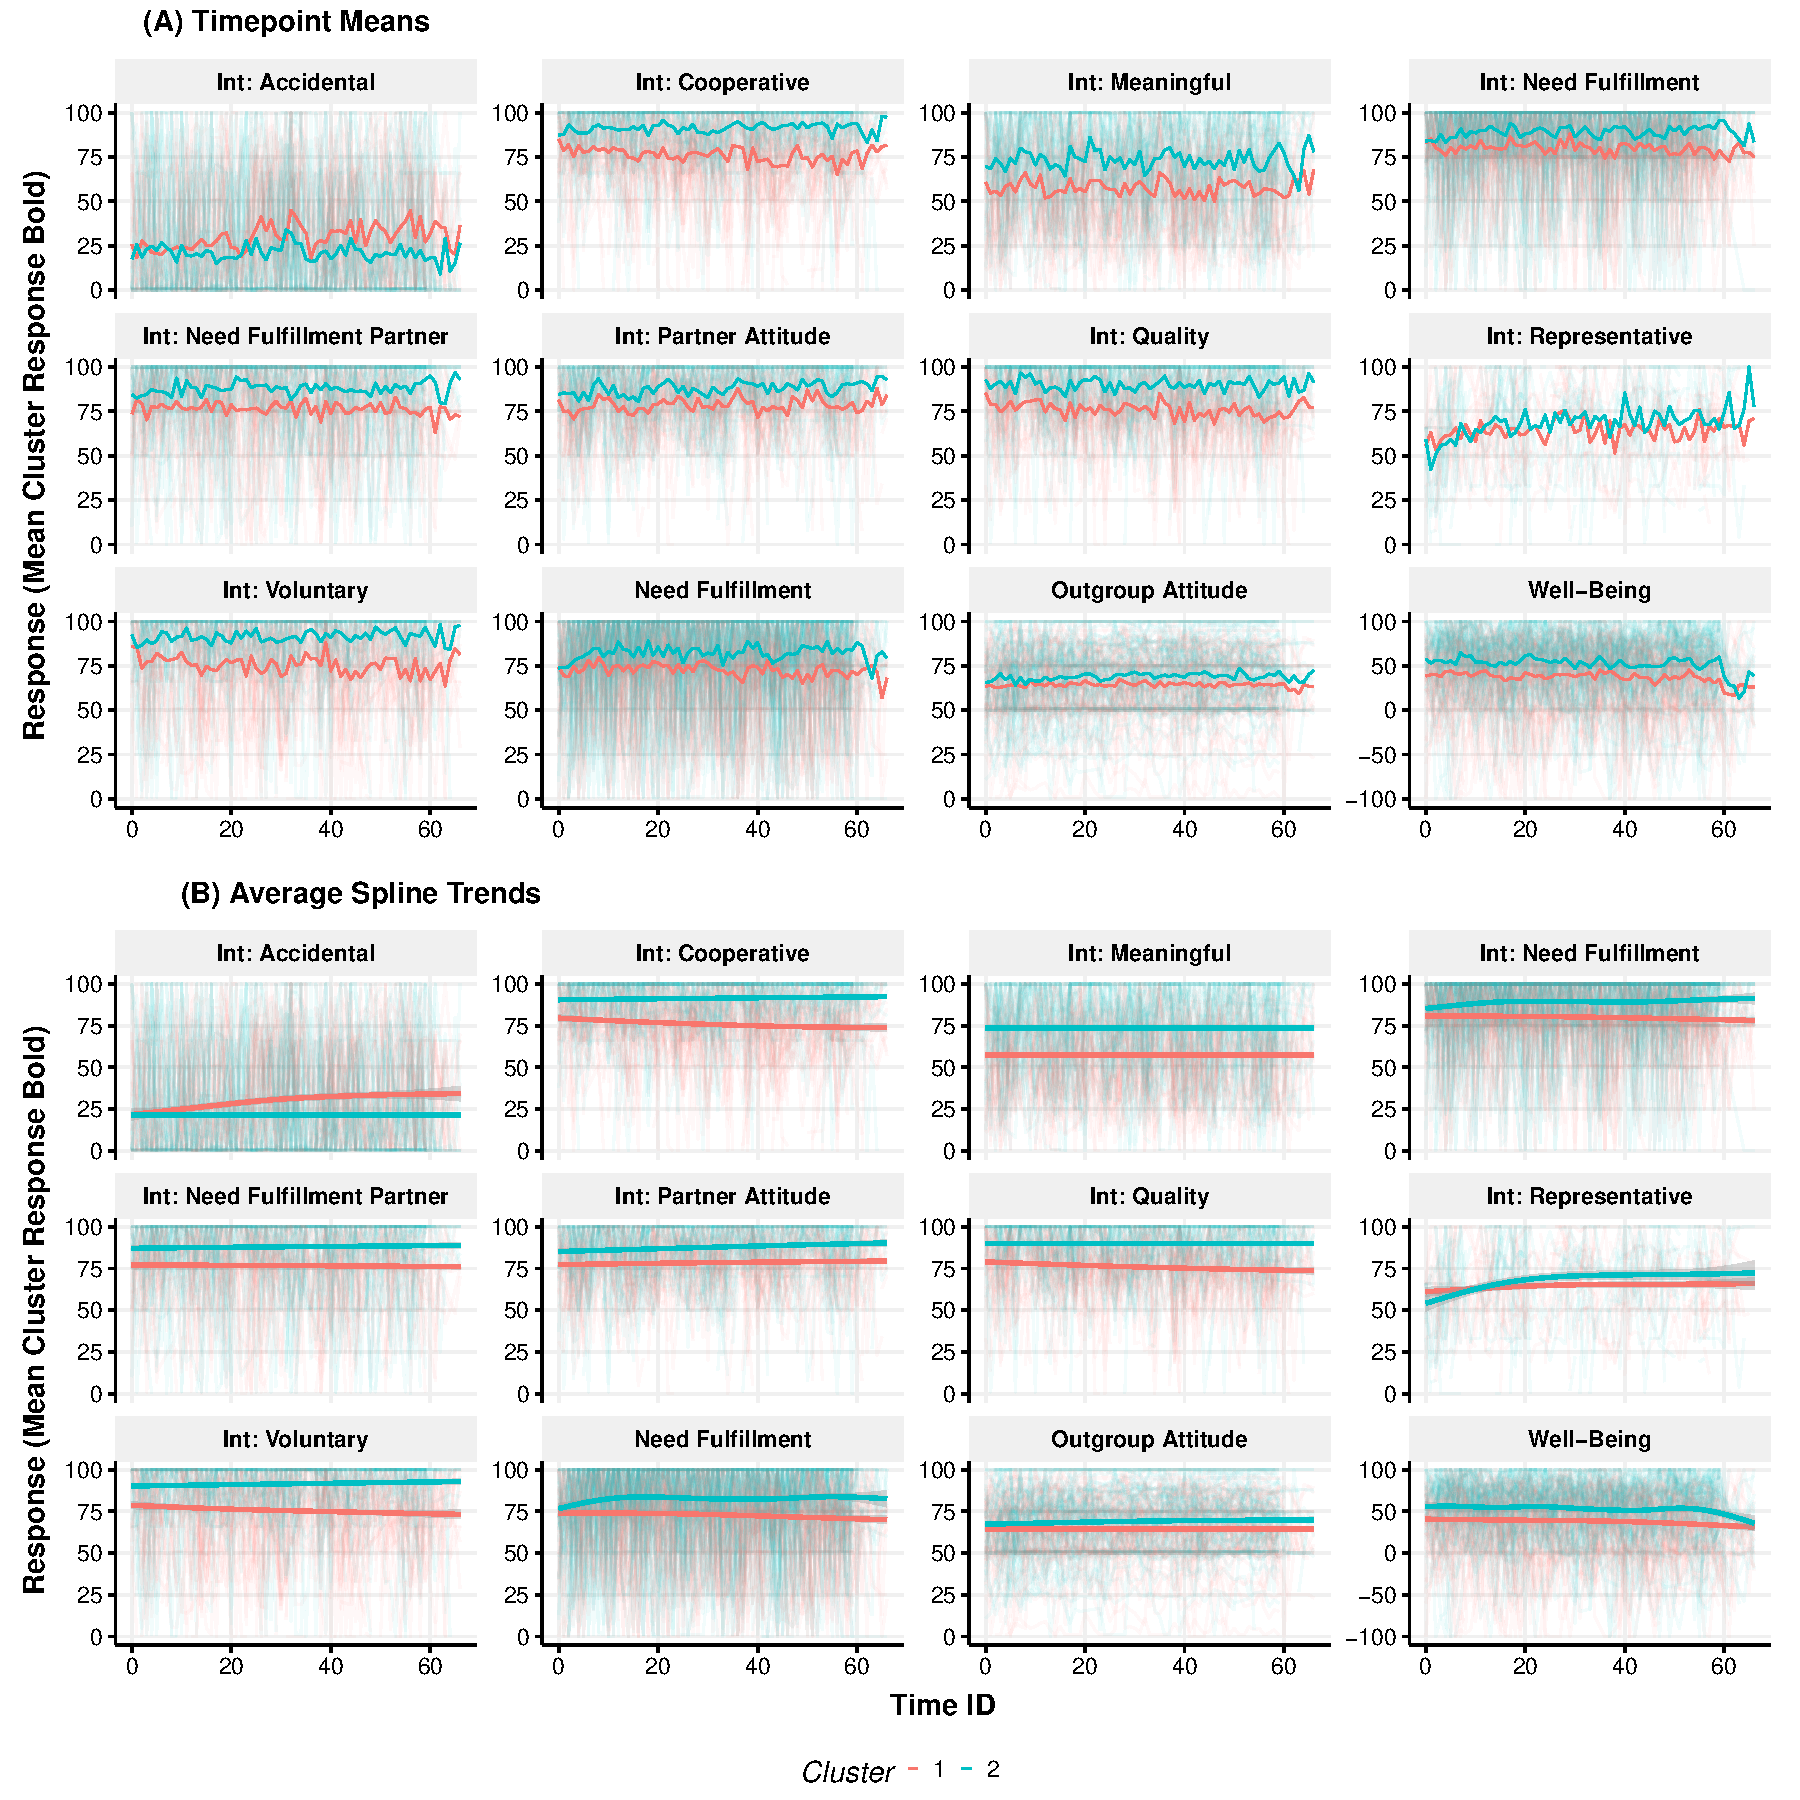
\includegraphics[width=\textwidth]{figures/clusterTsComb.pdf}
  \caption*{Note: \\
  Subplot (A) displays the variable cluster means at every measurement occasion. Subplot (B) shows the GAM spline for each cluster across the measurement occasions.}
\end{figure}
